\documentclass[12pt,a4paper]{article}
\usepackage[utf8]{inputenc}
\usepackage[margin=1in]{geometry}
\usepackage{amsmath}
\usepackage{amsfonts}
\usepackage{amssymb}
\usepackage{graphicx}
\usepackage{listings}
\usepackage{xcolor}
\usepackage{fancyhdr}
\usepackage{titlesec}

% SQL syntax highlighting
\lstdefinestyle{sqlstyle}{
    language=SQL,
    basicstyle=\ttfamily\small,
    keywordstyle=\color{blue}\bfseries,
    commentstyle=\color{green!50!black},
    stringstyle=\color{red},
    numbers=left,
    numberstyle=\tiny\color{gray},
    numbersep=5pt,
    breaklines=true,
    breakatwhitespace=true,
    tabsize=2,
    showspaces=false,
    showstringspaces=false,
    frame=single,
    rulecolor=\color{gray!30},
    backgroundcolor=\color{gray!5}
}

\lstset{style=sqlstyle}

% Page setup
\pagestyle{fancy}
\fancyhf{}
\rhead{CSE 414 - Assignment 01}
\lhead{SQL practice}
\cfoot{\thepage}

% Title formatting
\titleformat{\section}{\Large\bfseries}{\thesection}{1em}{}
\titleformat{\subsection}{\large\bfseries}{\thesubsection}{1em}{}

\begin{document}

% Title Page
\begin{titlepage}
    \centering
    \vspace*{2cm}
    {\Huge\bfseries University of Chittagong}\\[0.5cm]
    {\Large Department of Computer Science \& Engineering}\\[0.5cm]
    {\large Database Systems Lab}\\[2cm]
    
    {\huge\bfseries Assignment 1}\\[0.5cm]
    {\LARGE Chapters 1-4 Practice Problems}\\[0.5cm]
    {\large CSE 414}\\[3cm]
    
    \begin{tabular}{ll}
        \Large \textbf{Submitted By:} & \Large Debashish Chakraborty\\\\
        & \Large ID: 23701034\\[2cm]
        \Large \textbf{Submitted To:} & \Large Dr. Rudra Pratap Deb Nath\\\\
        & \Large Associate Professor\\
    \end{tabular}\\[4cm]
    
    {\large February 27, 2025}
\end{titlepage}

\newpage
\tableofcontents
\newpage

\section{Chapter 1 Problems \& Solutions}

\subsection{Part 1}

\textbf{Problem 1.} The following SELECT statement executes successfully:
\begin{lstlisting}[style=sqlstyle]
SELECT last_name, job_id, salary AS Sal
FROM employees;
\end{lstlisting}

\textbf{Solution:} TRUE

\vspace{0.5cm}

\textbf{Problem 2.} The following SELECT statement executes successfully:
\begin{lstlisting}[style=sqlstyle]
SELECT *
FROM job_grades;
\end{lstlisting}

\textbf{Solution:} TRUE

\vspace{0.5cm}

\textbf{Problem 3.} There are four coding errors in the following statement. Can you identify them?
\begin{lstlisting}[style=sqlstyle]
SELECT employee_id, last_name
sal x 12 ANNUAL SALARY
FROM employees;
\end{lstlisting}

\textbf{Solution:}
The detected errors are:
\begin{enumerate}
    \item Column names with spaces must be written correctly - employee\_id and last\_name are invalid unless quoted.
    \item Missing commas between selected columns - There's no comma between last\_name and sal x 12 ANNUAL SALARY.
    \item Invalid expression syntax - sal x 12 is invalid. It should be salary * 12.
    \item Missing AS for alias (optional but recommended) - ANNUAL SALARY should be written as AS "ANNUAL SALARY" if you want a readable header.
\end{enumerate}

\vspace{0.5cm}

\subsection{Part 2}

\textbf{Problem 4.} Your first task is to determine the structure of the DEPARTMENTS table and its contents.
\begin{figure}[htbp]
  \centering
  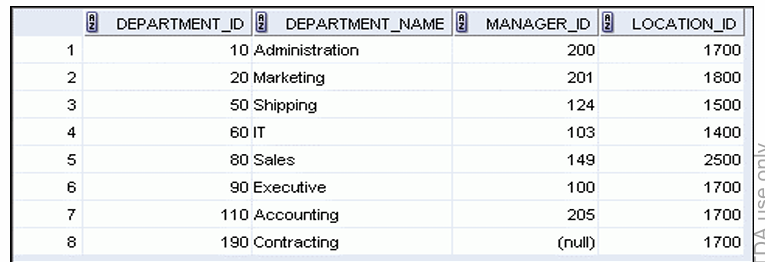
\includegraphics[width=0.7\textwidth]{Screenshots/14_2.png}
\end{figure}
\textbf{Solution:}
\begin{lstlisting}[style=sqlstyle]
DESC HR.EMPLOYEES;
\end{lstlisting}

Table structure:
\begin{verbatim}
Name                Null?    Type
--------------- -------- ------------
DEPARTMENT_ID   NOT NULL NUMBER(4)
DEPARTMENT_NAME NOT NULL VARCHAR2(30)
MANAGER_ID               NUMBER(6)
LOCATION_ID              NUMBER(4)
\end{verbatim}

\vspace{0.5cm}

\textbf{Problem 5.} The HR department wants a query to display the last name, job ID, hire date, and employee ID for each employee, with the employee ID appearing first. Provide an alias STARTDATE for the HIRE\_DATE column. Save your SQL statement to a file named lab\_01\_05.sql so that you can dispatch this file to the HR department.

\textbf{Solution:}
\begin{lstlisting}[style=sqlstyle]
SELECT employee_id, last_name, hire_date 
FROM HR.EMPLOYEES;
\end{lstlisting}

\vspace{0.5cm}

\textbf{Problem 6.} Test your query in the lab\_01\_05.sql file to ensure that it runs correctly.
\begin{figure}[htbp]
  \centering
  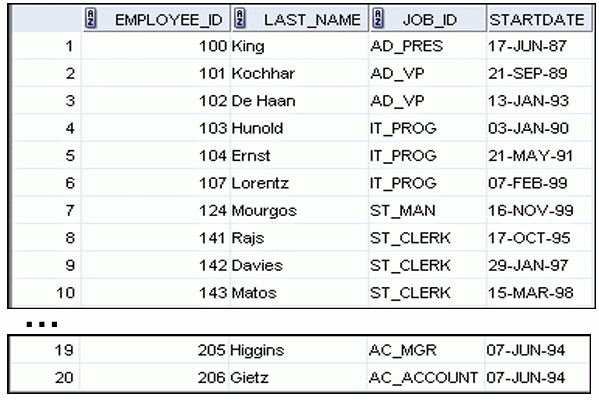
\includegraphics[width=0.7\textwidth]{Screenshots/16.png}
\end{figure}

\textbf{Solution:}
\begin{lstlisting}[style=sqlstyle]
SELECT employee_id, last_name, hire_date 
FROM HR.EMPLOYEES;
\end{lstlisting}

\vspace{0.5cm}

\textbf{Problem 7.} The HR department wants a query to display all unique job IDs from the EMPLOYEES table.


\textbf{Solution:}
\begin{lstlisting}[style=sqlstyle]
SELECT UNIQUE(job_id) 
FROM hr.employees;
\end{lstlisting}

\vspace{0.5cm}

\subsection{Part 3}

\textbf{Problem 8.} The HR department wants more descriptive column headings for its report on employees. Copy the statement from lab\_01\_05.sql to a new SQL Worksheet. Name the column headings Emp \#, Employee, Job, and Hire Date, respectively. Then run your query again.

\textbf{Solution:}
\begin{lstlisting}[style=sqlstyle]
SELECT employee_id AS "Emp #", 
       CONCAT(FIRST_NAME, ' ', LAST_NAME) AS "Employee", 
       job_id AS "Job", 
       hire_date AS "Hire Date" 
FROM hr.employees;
\end{lstlisting}

\vspace{0.5cm}

\textbf{Problem 9.} The HR department has requested a report of all employees and their job IDs. Display the last name concatenated with the job ID (separated by a comma and space) and name the column Employee and Title.

\begin{figure}[htbp]
  \centering
  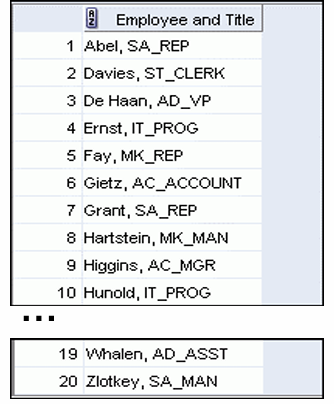
\includegraphics[width=0.4\textwidth]{Screenshots/19.png}
\end{figure}


\textbf{Solution:}
\begin{lstlisting}[style=sqlstyle]
SELECT LAST_NAME || ', ' || JOB_ID AS "Employee and Title"
FROM HR.EMPLOYEES;
\end{lstlisting}

\vspace{0.5cm}

\textbf{Problem 10.} To familiarize yourself with the data in the EMPLOYEES table, create a query to display all the data from that table. Separate each column output by a comma. Name the column title THE\_OUTPUT.

\begin{figure}[htbp]
  \centering
  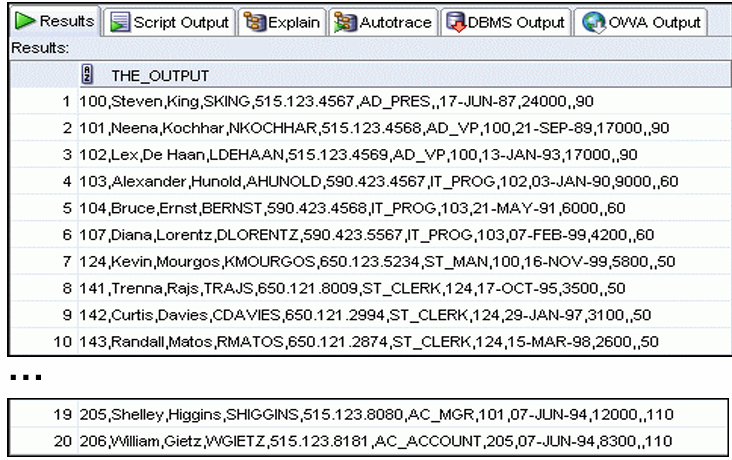
\includegraphics[width=0.5\textwidth]{Screenshots/110.png}
\end{figure}


\\\textbf{Solution:}
\begin{lstlisting}[style=sqlstyle]
SELECT
    EMPLOYEE_ID || ', ' ||
    FIRST_NAME || ', ' ||
    LAST_NAME || ', ' ||
    EMAIL || ', ' ||
    PHONE_NUMBER || ', ' ||
    TO_CHAR(HIRE_DATE, 'YYYY-MM-DD') || ', ' ||
    JOB_ID || ', ' ||
    SALARY || ', ' ||
    COMMISSION_PCT || ', ' ||
    MANAGER_ID || ', ' ||
    DEPARTMENT_ID AS "THE_OUTPUT"
FROM HR.EMPLOYEES;
\end{lstlisting}

\vspace{0.5cm}

\section{Chapter 2 Problems \& Solutions}

\textbf{Problem 1.} Because of budget issues, the HR department needs a report that displays the last name and salary of employees who earn more than \$12,000. Save your SQL statement as a file named lab\_02\_01.sql. Run your query.

\begin{figure}[htbp]
  \centering
  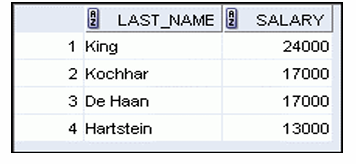
\includegraphics[width=0.5\textwidth]{Screenshots/21.png}
\end{figure}\\

\textbf{Solution:}
\begin{lstlisting}[style=sqlstyle]
SELECT LAST_NAME, SALARY
FROM HR.EMPLOYEES
WHERE SALARY > 12000;
\end{lstlisting}

\vspace{0.5cm}

\textbf{Problem 2.} Open a new SQL Worksheet. Create a report that displays the last name and department number for employee number 176. Run the query.
\begin{figure}[htbp]
  \centering
  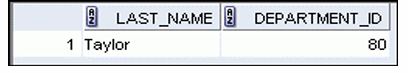
\includegraphics[width=0.5\textwidth]{Screenshots/22.png}
\end{figure}\\

\textbf{Solution:}
\begin{lstlisting}[style=sqlstyle]
SELECT LAST_NAME, DEPARTMENT_ID
FROM HR.EMPLOYEES
WHERE EMPLOYEE_ID = 176;
\end{lstlisting}

\vspace{0.5cm}

\textbf{Problem 3.} The HR department needs to find high-salary and low-salary employees. Modify lab\_02\_01.sql to display the last name and salary for any employee whose salary is not in the range of \$5,000 to \$12,000. Save your SQL statement as lab\_02\_03.sql.

\begin{figure}[htbp]
  \centering
  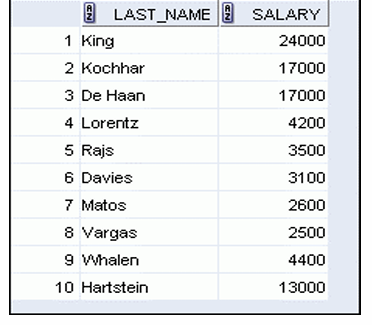
\includegraphics[width=0.5\textwidth]{Screenshots/23.png}
\end{figure}\\

\textbf{Solution:}
\begin{lstlisting}[style=sqlstyle]
SELECT LAST_NAME, SALARY
FROM HR.EMPLOYEES
WHERE SALARY NOT BETWEEN 5000 AND 12000;
\end{lstlisting}

\vspace{0.5cm}

\textbf{Problem 4.} Create a report to display the last name, job ID, and hire date for employees with the last names of Matos and Taylor. Order the query in ascending order by the hire date.
\begin{figure}[htbp]
  \centering
  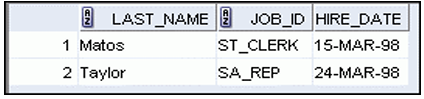
\includegraphics[width=0.5\textwidth]{Screenshots/24.png}
\end{figure}\\
\textbf{Solution:}
\begin{lstlisting}[style=sqlstyle]
SELECT LAST_NAME, JOB_ID, HIRE_DATE
FROM HR.EMPLOYEES
WHERE LAST_NAME IN ('Matos', 'Taylor')
ORDER BY HIRE_DATE ASC;
\end{lstlisting}

\vspace{0.5cm}

\textbf{Problem 5.} Display the last name and department ID of all employees in departments 20 or 50 in ascending alphabetical order by name.
\begin{figure}[htbp]
  \centering
  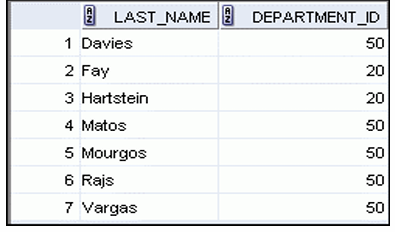
\includegraphics[width=0.5\textwidth]{Screenshots/25.png}
\end{figure}\\
\textbf{Solution:}
\begin{lstlisting}[style=sqlstyle]
SELECT LAST_NAME, DEPARTMENT_ID
FROM HR.EMPLOYEES
WHERE DEPARTMENT_ID IN (20, 50)
ORDER BY LAST_NAME ASC;
\end{lstlisting}

\vspace{0.5cm}

\textbf{Problem 6.} Modify lab\_02\_03.sql to display the last name and salary of employees who earn between \$5,000 and \$12,000, and are in department 20 or 50. Label the columns Employee and Monthly Salary, respectively. Resave lab\_02\_03.sql as lab\_02\_06.sql. Run the statement in lab\_02\_06.sql.
\begin{figure}[htbp]
  \centering
  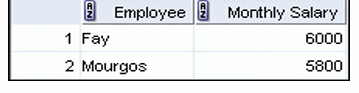
\includegraphics[width=0.5\textwidth]{Screenshots/26.png}
\end{figure}\\
\textbf{Solution:}
\begin{lstlisting}[style=sqlstyle]
SELECT LAST_NAME AS "Employee",
       SALARY AS "Monthly Salary"
FROM HR.EMPLOYEES
WHERE SALARY BETWEEN 5000 AND 12000
  AND DEPARTMENT_ID IN (20, 50);
\end{lstlisting}

\vspace{0.5cm}

\textbf{Problem 7.} The HR department needs a report that displays the last name and hire date for all employees who were hired in 1994.
\begin{figure}[htbp]
  \centering
  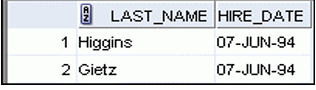
\includegraphics[width=0.5\textwidth]{Screenshots/27.png}
\end{figure}\\
\textbf{Solution:}
\begin{lstlisting}[style=sqlstyle]
SELECT LAST_NAME, HIRE_DATE
FROM HR.EMPLOYEES
WHERE TO_CHAR(HIRE_DATE, 'YYYY') = '1994';
\end{lstlisting}

\vspace{0.5cm}

\textbf{Problem 8.} Create a report to display the last name and job title of all employees who do not have a manager.
\begin{figure}[htbp]
  \centering
  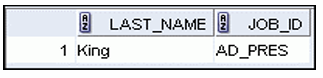
\includegraphics[width=0.5\textwidth]{Screenshots/28.png}
\end{figure}\\
\textbf{Solution:}
\begin{lstlisting}[style=sqlstyle]
SELECT LAST_NAME, JOB_ID
FROM HR.EMPLOYEES
WHERE MANAGER_ID IS NULL;
\end{lstlisting}

\vspace{0.5cm}

\textbf{Problem 9.} Create a report to display the last name, salary, and commission of all employees who earn commissions. Sort data in descending order of salary and commissions. Use the column's numeric position in the ORDER BY clause.
\begin{figure}[htbp]
  \centering
  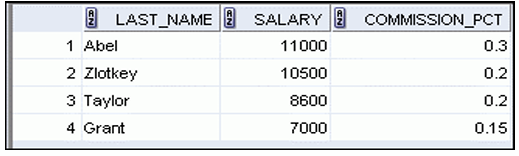
\includegraphics[width=0.5\textwidth]{Screenshots/29.png}
\end{figure}\\
\textbf{Solution:}
\begin{lstlisting}[style=sqlstyle]
SELECT LAST_NAME, SALARY, COMMISSION_PCT
FROM HR.EMPLOYEES
WHERE COMMISSION_PCT IS NOT NULL
ORDER BY 2 DESC, 3 DESC;
\end{lstlisting}

\vspace{0.5cm}

\textbf{Problem 10.} Members of the HR department want to have more flexibility with the queries that you are writing. They would like a report that displays the last name and salary of employees who earn more than an amount that the user specifies after a prompt. Save this query to a file named lab\_02\_10.sql. If you enter 12000 when prompted, the report displays the following results:

\textbf{Solution:}
\begin{lstlisting}[style=sqlstyle]
-- lab_02_10.sql
SELECT last_name, salary
FROM HR.EMPLOYEES
WHERE salary > &amount;
\end{lstlisting}

\vspace{0.5cm}

\\ \\

\textbf{Problem 11.} The HR department wants to run reports based on a manager. Create a query that prompts the user for a manager ID and generates the employee ID, last name, salary, and department for that manager's employees. The HR department wants the ability to sort the report on a selected column.
\begin{figure}[htbp]
  \centering
  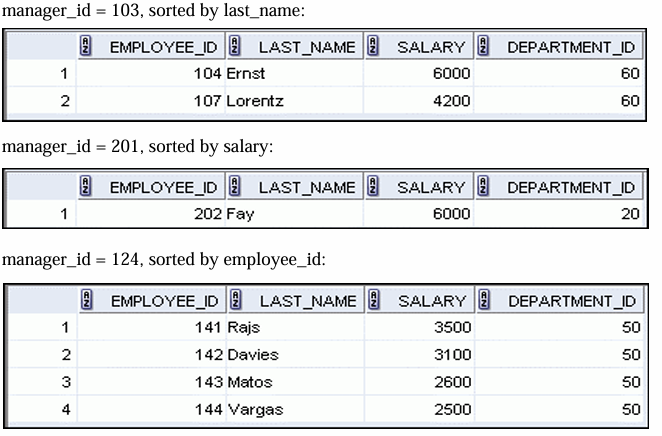
\includegraphics[width=0.5\textwidth]{Screenshots/211.png}
\end{figure}\\
\textbf{Solution:} We can create a flexible query that prompts for both the manager ID and the sorting column. Here's how you'd do it in Oracle SQL*Plus (which supports substitution variables):

\begin{lstlisting}[style=sqlstyle]
SELECT employee_id, last_name, salary, department_id
FROM HR.EMPLOYEES
WHERE manager_id = &manager_id
ORDER BY &sort_column;
\end{lstlisting}

Examples:
\begin{itemize}
    \item manager\_id = 103, sorted by last\_name:
    \begin{verbatim}
    Enter value for manager_id: 103
    Enter value for sort_column: last_name
    \end{verbatim}
    
    \item manager\_id = 201, sorted by salary:
    \begin{verbatim}
    Enter value for manager_id: 201
    Enter value for sort_column: salary
    \end{verbatim}
    
    \item manager\_id = 124, sorted by employee\_id:
    \begin{verbatim}
    Enter value for manager_id: 124
    Enter value for sort_column: employee_id
    \end{verbatim}
\end{itemize}

\vspace{0.5cm}

\textbf{Problem 12.} Display all employee last names in which the third letter of the name is "a."
\begin{figure}[htbp]
  \centering
  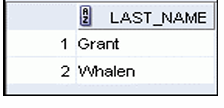
\includegraphics[width=0.4\textwidth]{Screenshots/212.png}
\end{figure}\\
\textbf{Solution:}
\begin{lstlisting}[style=sqlstyle]
SELECT last_name
FROM HR.EMPLOYEES
WHERE last_name LIKE '__a%';
\end{lstlisting}

\vspace{0.5cm}

\textbf{Problem 13.} Display the last names of all employees who have both an "a" and an "e" in their last name.
\begin{figure}[htbp]
  \centering
  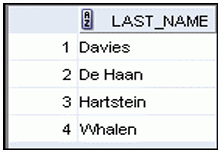
\includegraphics[width=0.4\textwidth]{Screenshots/213.png}
\end{figure}\\
\textbf{Solution:}
\begin{lstlisting}[style=sqlstyle]
SELECT last_name
FROM HR.EMPLOYEES
WHERE last_name LIKE '%a%' AND last_name LIKE '%e%';
\end{lstlisting}

\vspace{0.5cm}

\textbf{Problem 14.} Display the last name, job, and salary for all employees whose jobs are either those of a sales representative or of a stock clerk, and whose salaries are not equal to \$2,500, \$3,500, or \$7,000.
\begin{figure}[htbp]
  \centering
  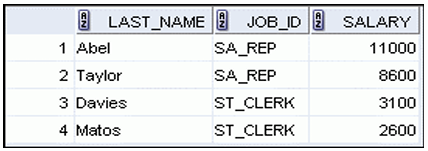
\includegraphics[width=0.5\textwidth]{Screenshots/214.png}
\end{figure}\\
\textbf{Solution:}
\begin{lstlisting}[style=sqlstyle]
SELECT last_name, job_id, salary
FROM HR.EMPLOYEES
WHERE job_id IN ('SA_REP', 'ST_CLERK')
  AND salary NOT IN (2500, 3500, 7000);
\end{lstlisting}

\vspace{0.5cm}

\textbf{Problem 15.} Modify lab\_02\_06.sql to display the last name, salary, and commission for all employees whose commission is 20\%. Resave lab\_02\_06.sql as lab\_02\_15.sql. Rerun the statement in lab\_02\_15.sql.
\begin{figure}[htbp]
  \centering
  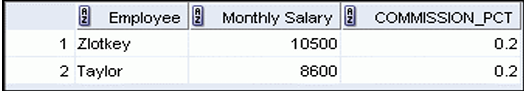
\includegraphics[width=0.5\textwidth]{Screenshots/215.png}
\end{figure}\\
\textbf{Solution:}
\begin{lstlisting}[style=sqlstyle]
SELECT last_name, salary, commission_pct
FROM HR.EMPLOYEES
WHERE commission_pct = 0.2;
\end{lstlisting}

\vspace{0.5cm}

\section{Chapter 3 Problems \& Solutions}

\textbf{Problem 1.} Write a query to display the system date. Label the column as Date.
\begin{figure}[htbp]
  \centering
  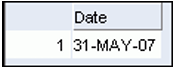
\includegraphics[width=0.3\textwidth]{Screenshots/31.png}
\end{figure}\\
Note: If your database is remotely located in a different time zone, the output will be the date for the operating system on which the database resides.

\textbf{Solution:}
\begin{lstlisting}[style=sqlstyle]
SELECT SYSDATE AS "Date"
FROM dual;
\end{lstlisting}

\vspace{0.5cm}

\textbf{Problem 2.} The HR department needs a report to display the employee number, last name, salary, and salary increased by 15.5\% (expressed as a whole number) for each employee. Label the column New Salary. Save your SQL statement in a file named lab\_03\_02.sql.

\textbf{Solution:}
\begin{lstlisting}[style=sqlstyle]
-- lab_03_02.sql
SELECT employee_id, last_name, salary,
       FLOOR(salary * 1.155) AS "New Salary"
FROM HR.EMPLOYEES;
\end{lstlisting}

\vspace{0.5cm}

\textbf{Problem 3.} Run your query in the lab\_03\_02.sql file.

\textbf{Solution:}
\begin{lstlisting}[style=sqlstyle]
-- lab_03_02.sql
SELECT employee_id, last_name, salary,
       FLOOR(salary * 1.155) AS "New Salary"
FROM HR.EMPLOYEES;
\end{lstlisting}

Sample output:
\begin{verbatim}
EMPLOYEE_ID LAST_NAME  SALARY  NEW SALARY
100         King       24000   27720
101         Kochhar    17000   19635
102         De Haan    17000   19635
103         Hunold      9000   10395
104         Ernst       6000    6930
...         ...         ...     ...
\end{verbatim}

\vspace{0.5cm}

\textbf{Problem 4.} Modify your query lab\_03\_02.sql to add a column that subtracts the old salary from the new salary. Label the column Increase. Save the contents of the file as lab\_03\_04.sql. Run the revised query.
\begin{figure}[htbp]
  \centering
  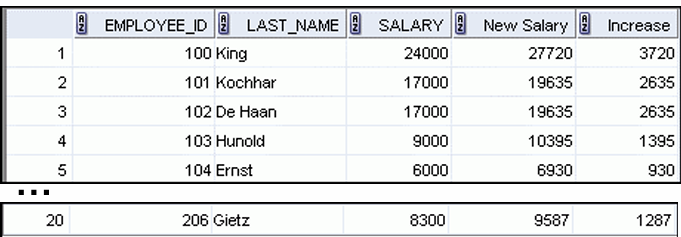
\includegraphics[width=0.5\textwidth]{Screenshots/34.png}
\end{figure}\\
\textbf{Solution:}
\begin{lstlisting}[style=sqlstyle]
-- lab_03_04.sql
SELECT employee_id, last_name, salary,
       FLOOR(salary * 1.155) AS "New Salary",
       FLOOR(salary * 1.155) - salary AS "Increase"
FROM HR.EMPLOYEES;
\end{lstlisting}

\vspace{0.5cm}

\textbf{Problem 5.} Write a query that displays the last name (with the first letter in uppercase and all the other letters in lowercase) and the length of the last name for all employees whose name starts with the letters "J," "A," or "M." Give each column an appropriate label. Sort the results by the employees' last names.
\begin{figure}[htbp]
  \centering
  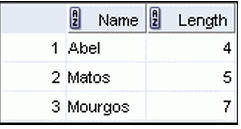
\includegraphics[width=0.3\textwidth]{Screenshots/35_1.png}
\end{figure}\\
\textbf{Solution:}
\begin{lstlisting}[style=sqlstyle]
SELECT INITCAP(last_name) AS "Formatted Last Name",
       LENGTH(last_name) AS "Name Length"
FROM HR.EMPLOYEES
WHERE UPPER(SUBSTR(last_name, 1, 1)) IN ('J', 'A', 'M')
ORDER BY last_name;
\end{lstlisting}

Rewrite the query so that the user is prompted to enter a letter that the last name starts with. For example, if the user enters "H" (capitalized) when prompted for a letter, then the output should show all employees whose last name starts with the letter "H."
\begin{figure}[htbp]
  \centering
  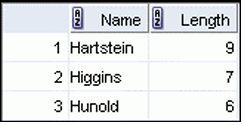
\includegraphics[width=0.3\textwidth]{Screenshots/35_2.png}
\end{figure}\\
\begin{lstlisting}[style=sqlstyle]
SELECT INITCAP(last_name) AS "Formatted Last Name",
       LENGTH(last_name) AS "Name Length"
FROM HR.EMPLOYEES
WHERE UPPER(SUBSTR(last_name, 1, 1)) = UPPER('&start_letter')
ORDER BY last_name;
\end{lstlisting}

Modify the query such that the case of the entered letter does not affect the output. The entered letter must be capitalized before being processed by the SELECT query.
\begin{figure}[htbp]
  \centering
  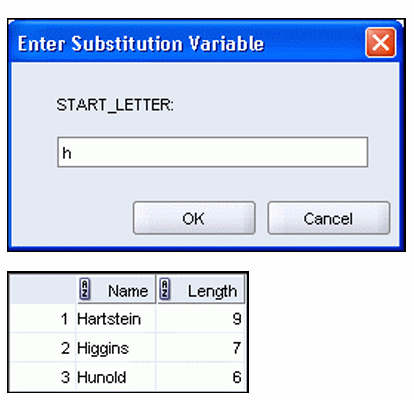
\includegraphics[width=0.3\textwidth]{Screenshots/35_3.png}
\end{figure}\\
\\
\\\begin{lstlisting}[style=sqlstyle]
SELECT INITCAP(last_name) AS "Formatted Last Name",
       LENGTH(last_name) AS "Name Length"
FROM HR.EMPLOYEES
WHERE UPPER(SUBSTR(last_name, 1, 1)) = UPPER('&letter')
ORDER BY last_name;
\end{lstlisting}

\vspace{0.5cm}

\textbf{Problem 6.} The HR department wants to find the duration of employment for each employee. For each employee, display the last name and calculate the number of months between today and the date on which the employee was hired. Label the column as MONTHS\_WORKED. Order your results by the number of months employed. Round the number of months up to the closest whole number.

\textbf{Solution:}
\begin{lstlisting}[style=sqlstyle]
SELECT last_name,
       CEIL(MONTHS_BETWEEN(SYSDATE, hire_date)) AS "MONTHS_WORKED"
FROM HR.EMPLOYEES
ORDER BY "MONTHS_WORKED";
\end{lstlisting}

\vspace{0.5cm}

\textbf{Problem 7.} Create a query to display the last name and salary for all employees. Format the salary to be 15 characters long, left-padded with the \$ symbol. Label the column as SALARY.
\begin{figure}[htbp]
  \centering
  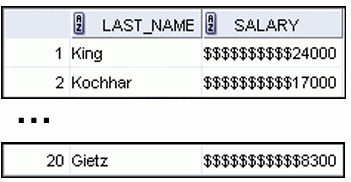
\includegraphics[width=0.3\textwidth]{Screenshots/37.png}
\end{figure}\\
\textbf{Solution:}
\begin{lstlisting}[style=sqlstyle]
SELECT last_name,
       LPAD(salary, 15, '$') AS "SALARY"
FROM HR.EMPLOYEES;
\end{lstlisting}

\vspace{0.5cm}

\textbf{Problem 8.} Create a query that displays the first eight characters of the employees' last names and indicates the amounts of their salaries with asterisks. Each asterisk signifies a thousand dollars. Sort the data in descending order of salary. Label the column as EMPLOYEES\_AND\_THEIR\_SALARIES.
\begin{figure}[htbp]
  \centering
  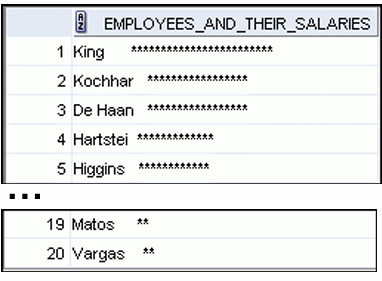
\includegraphics[width=0.3\textwidth]{Screenshots/38.png}
\end{figure}\\
\textbf{Solution:}
\begin{lstlisting}[style=sqlstyle]
SELECT RPAD(SUBSTR(last_name, 1, 8), 8, ' ') || ' ' ||
       RPAD('*', FLOOR(salary / 1000), '*') AS "EMPLOYEES_AND_THEIR_SALARIES"
FROM HR.EMPLOYEES
ORDER BY salary DESC;
\end{lstlisting}

\vspace{0.5cm}

\textbf{Problem 9.} Create a query to display the last name and the number of weeks employed for all employees in department 90. Label the number of weeks column as TENURE. Truncate the number of weeks value to 0 decimal places. Show the records in descending order of the employee's tenure. Note: The TENURE value will differ as it depends on the date on which you run the query.
\begin{figure}[htbp]
  \centering
  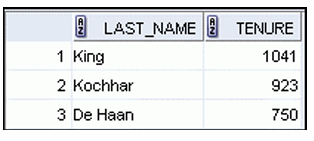
\includegraphics[width=0.3\textwidth]{Screenshots/39.png}
\end{figure}\\
\textbf{Solution:}
\begin{lstlisting}[style=sqlstyle]
SELECT last_name,
       TRUNC((SYSDATE - hire_date) / 7) AS TENURE
FROM HR.EMPLOYEES
WHERE department_id = 90
ORDER BY TENURE DESC;
\end{lstlisting}

\vspace{0.5cm}

\section{Chapter 4 Problems \& Solutions}

\textbf{Problem 1.} Create a report that produces the following for each employee: $<$employee last name$>$ earns $<$salary$>$ monthly but wants $<$3 times salary.$>$ Label the column Dream Salaries.
\begin{figure}[htbp]
  \centering
  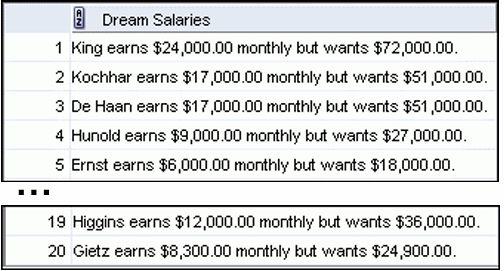
\includegraphics[width=0.5\textwidth]{Screenshots/41.png}
\end{figure}\\
\textbf{Solution:}
\begin{lstlisting}[style=sqlstyle]
SELECT last_name || ' earns ' || salary || ' monthly but wants ' || 
       (salary * 3) || '.' AS "Dream Salaries"
FROM HR.EMPLOYEES;
\end{lstlisting}

\vspace{0.5cm}

\textbf{Problem 2.} Display each employee's last name, hire date, and salary review date, which is the first Monday after six months of service. Label the column REVIEW. Format the dates to appear in the format similar to "Monday, the Thirty-First of July, 2000."
\begin{figure}[htbp]
  \centering
  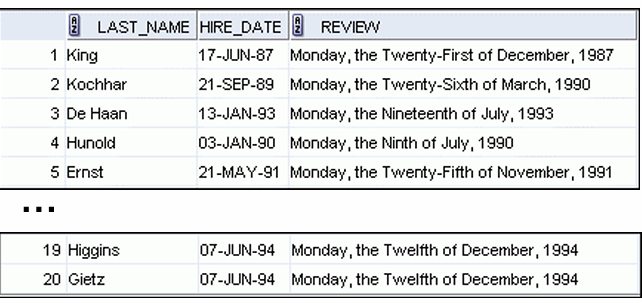
\includegraphics[width=0.5\textwidth]{Screenshots/42.png}
\end{figure}\\
\textbf{Solution:}
\begin{lstlisting}[style=sqlstyle]
SELECT last_name,
       TO_CHAR(hire_date, 'Day, "the" Ddspth "of" Month, YYYY') AS "Hire Date",
       TO_CHAR(
           NEXT_DAY(ADD_MONTHS(hire_date, 6) - 1, 'MONDAY'),
           'Day, "the" Ddspth "of" Month, YYYY'
       ) AS "Review"
FROM HR.EMPLOYEES;
\end{lstlisting}

\vspace{0.5cm}

\textbf{Problem 3.} Display the last name, hire date, and day of the week on which the employee started. Label the column DAY. Order the results by the day of the week, starting with Monday.
\begin{figure}[htbp]
  \centering
  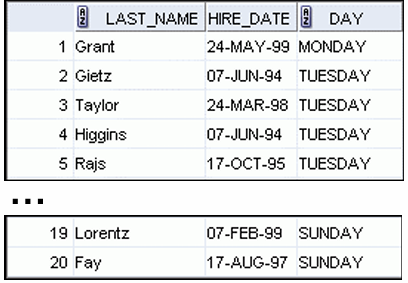
\includegraphics[width=0.3\textwidth]{Screenshots/43.png}
\end{figure}\\
\textbf{Solution:}
\begin{lstlisting}[style=sqlstyle]
SELECT last_name,
       hire_date,
       TO_CHAR(hire_date, 'Day') AS DAY
FROM HR.EMPLOYEES
ORDER BY TO_CHAR(hire_date, 'D');
\end{lstlisting}

\vspace{0.5cm}

\textbf{Problem 4.} Create a query that displays the employees' last names and commission amounts. If an employee does not earn commission, show "No Commission." Label the column COMM.
\begin{figure}[htbp]
  \centering
  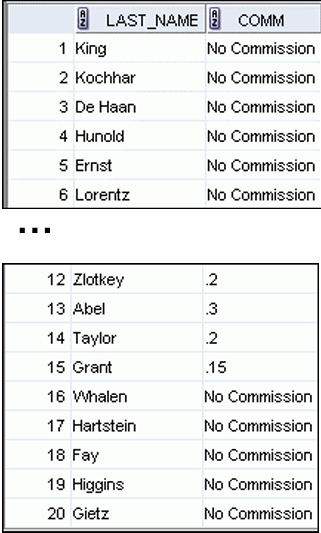
\includegraphics[width=0.3\textwidth]{Screenshots/44.png}
\end{figure}\\
\textbf{Solution:}
\begin{lstlisting}[style=sqlstyle]
SELECT last_name,
       NVL(TO_CHAR(commission_pct), 'No Commission') AS COMM
FROM HR.EMPLOYEES;
\end{lstlisting}

\vspace{0.5cm}

\textbf{Problem 5.} Using the DECODE function, write a query that displays the grade of all employees based on the value of the column JOB\_ID, using the following data:

\textbf{Solution:}
\begin{lstlisting}[style=sqlstyle]
SELECT last_name,
       job_id,
       DECODE(job_id,
           'AD_PRES', 'A',
           'ST_MAN', 'B',
           'IT_PROG', 'C',
           'SA_REP', 'D',
           'ST_CLERK','E',
           '0') AS GRADE
FROM HR.EMPLOYEES;
\end{lstlisting}
\begin{figure}[htbp]
  \centering
  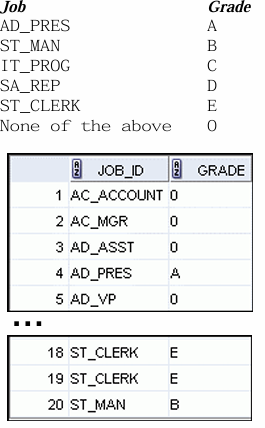
\includegraphics[width=0.3\textwidth]{Screenshots/45.png}
\end{figure}\\


\textbf{Problem 6.} Rewrite the statement in the preceding exercise using the CASE syntax.
\begin{figure}[htbp]
  \centering
  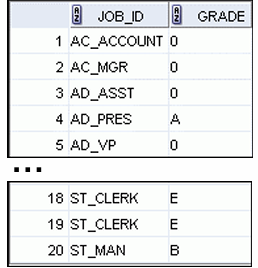
\includegraphics[width=0.2\textwidth]{Screenshots/46.png}
\end{figure}\\
\textbf{Solution:}
\begin{lstlisting}[style=sqlstyle]
SELECT last_name,
       job_id,
       CASE job_id
           WHEN 'AD_PRES' THEN 'A'
           WHEN 'ST_MAN' THEN 'B'
           WHEN 'IT_PROG' THEN 'C'
           WHEN 'SA_REP' THEN 'D'
           WHEN 'ST_CLERK' THEN 'E'
           ELSE '0'
       END AS GRADE
FROM HR.EMPLOYEES;
\end{lstlisting}

\vspace{0.5cm}

\end{document}



